\documentclass[twocolumn,english]{article}
\usepackage[latin9]{inputenc}
\usepackage[landscape]{geometry}
\geometry{verbose,tmargin=0.5in,bmargin=0.75in,lmargin=0.5in,rmargin=0.5in}
\usepackage{float}
\usepackage{booktabs}
\usepackage{graphicx}

\makeatletter

\providecommand{\tabularnewline}{\\}

\setlength{\columnsep}{0.25in}
\usepackage{xcolor}
\usepackage{textcomp}
\usepackage{listings}
\lstset{
  language=SQL,
  tabsize=2,
  frame=single,
  basicstyle=\small\ttfamily,
  keepspaces=true,
  moredelim=[is][\underbar]{*}{*},
}

\makeatother

\usepackage{babel}
\usepackage{listings}
\renewcommand{\lstlistingname}{Listing}

\begin{document}

\title{Reference Sheet for CO130 Databases}


\date{Spring 2017}

\maketitle

\section{Benefits of Databases}
\begin{enumerate}
\item Organised and efficient.
\item Minimise data duplication.
\item Support concurrent actions.
\item Support multiple users, controls who can access which data.
\item Support recovery from failures.
\end{enumerate}

\subsection{Transactions}
\begin{enumerate}
\item \emph{Atomicity}: if one part fails, whole transaction fails.
\item \emph{Consistency}: must not leave database in inconsistent state.
\item \emph{Isolation}: executed as if no other transaction is occurring.
\item \emph{Durability}: Results of successful transactions not lost.
\end{enumerate}

\section{Relational Model}
\begin{enumerate}
\item \emph{Database}: one or more relations.
\item \emph{Database schema}: schemas for all relations.
\item \emph{Relation}: heading and body: set of tuples of the form $\left(A_{1}:S_{1}=V_{1},\dots,A_{n}:S_{n}=V_{n}\right)$.
\item \emph{Relation schema}: name of relation and heading.
\item \emph{Heading}: unordered set of attributes (names and types).
\item \emph{Body}: unnordered set of tuples (sets of attribute values).
\end{enumerate}

\subsection{Entity-Relationship Digrams}
\begin{enumerate}
\item \emph{Entity sets} (rectangles): distinguishable entities tht share
same properties.
\item \emph{Relationship} (diamonds): captures how two or more entity sets
are related.
\item \emph{Attributes} (circles): property of entity, primary key attributes
underlined.
\end{enumerate}

\subsubsection{Complex Attributes}
\begin{enumerate}
\item \emph{Composite} (tree): subdivided e.g. address into road, city,
postcode.
\item \emph{Multivalued} (double border): set of values e.g. several phones.
\item \emph{Derived} (dotted line and border): computed from other values
e.g. age from DoB.
\end{enumerate}

\subsubsection{Cardinality Constraints and Entity Set Participation}
\begin{enumerate}
\item \emph{One-to-one}, \emph{one-to-many}, \emph{many-to-many}: add labels
1 1, 1 N, and M N to relationship respectively.
\item \emph{Total participation}: use double line, requires all entities
to participate in a relationship.
\item \emph{Participation bounds}: use .. notation in labels.
\end{enumerate}

\subsubsection{Fan Traps and Chasm Traps}

\emph{Fan traps}: ambiguous paths exist between entities. Can be solved
by changing structure (e.g. staff - dept - faculty).

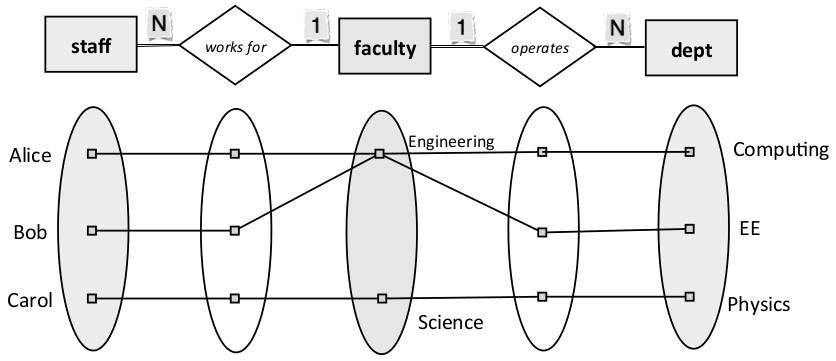
\includegraphics[scale=0.2]{img/fan}

\noindent \emph{Chasm traps}: suggests a relationship between entities
but one doesn't exist. Can be solved by adding a new relationship
(e.g. between dept and PC).

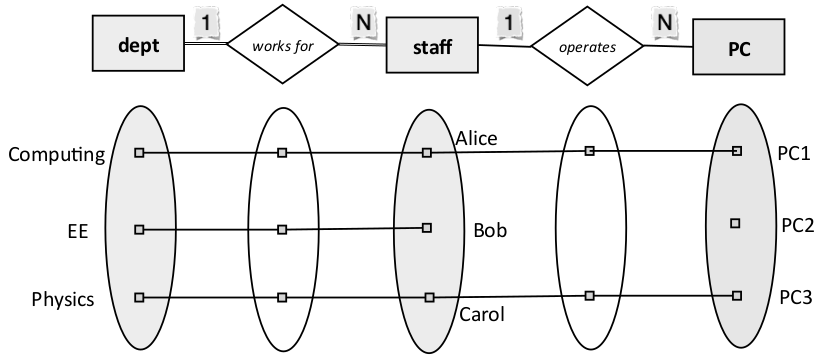
\includegraphics[scale=0.2]{img/chasm}


\subsubsection{More relationships}
\begin{enumerate}
\item \emph{Multiway relationships}: can have relationships between more
than two entity sets.
\item \emph{Roles}: one entity set can have more than one role (e.g. prequel
and sequel), draw multiple lines and label.
\item \emph{is-a relationships}: hollow arrow head, can form hierarchies.
\end{enumerate}

\subsubsection{More Entities}

\emph{Weak entities} (double rectangle, double diamond): cannot be
uniquely identified on own attributes and requires a strong entity
to exist. Identified using primary key of strong entity and one ore
more attributes of itself (dotted underlined). E.g. room cannot exist
without building that contains it.


\subsection{Relation Schemas from ER Models}


\subsubsection{Joins and Keys}
\begin{enumerate}
\item Primary key: uniquely identifies tuple
\item Foreign key: primary key used in different table
\end{enumerate}

\subsubsection{Entity Sets and attributes}

Mapped directly to realtion with the same attributes. E.g.

\begin{lstlisting}
actor(*ID*, firstname, lastname, housno, roadname, city)
actor_cars(*actorID*, *carID*)

create table actor (
	ID           int,
	firstname    varchar(30),
	lastname     varchar(30),
	houseno      int,
	roadname     varchar(30),
	city         varchar(40),

	primary key (ID)
)

create table actor_cars (
	actorID      int,
	carID        varchar(10),
	
	primary key (actorID, carID),
	foreign key (actorID) references actor.ID
)
\end{lstlisting}

\begin{enumerate}
\item \emph{Composite attributes}: flatten to contain only simple attributes.
\item \emph{Multivalued attributes}: own relation mapped back to entity
set using foreign key.
\item \emph{Derived attributes}: not supported by relational model.
\end{enumerate}

\paragraph{Weak Entity Sets}

Mapped to its own relation and attributes but includes primary key
of strong attribute with on delete cascade constraint.

\subsubsection{Relationships}

\emph{Many-to-many}: new relation with two foreign keys. E.g.

\begin{lstlisting}
person(*ID*, otherattributes)
car(*regno*, otherattributes)
drive(*personID*, *regno*, otherattributes)

create table drive (
	personID    varchar(10),
	regno       varchar(12),

	primary key (personID, regno),
	foreign key (personID) references person.ID on delete.cascade,
	foreign key (regno) references car.regno on delete.cascade
)
\end{lstlisting}


\noindent \emph{One-to-many} and \emph{one-to-one}: directly include
primary key of the One relation as foreign key in the Many relation.
E.g.

\begin{lstlisting}
person(*ID*, otherattributes)
car(*regno*, personID, otherattributes)

create table car (
	regno       varchar(12),
	personID    varchar(10),

	primary key (regno),
	foreign key (personID) references person.ID
)
\end{lstlisting}



\paragraph{Multiway Relationships}

Include primary keys from all entity sets of foreign keys. Primary
key is formed by foreign keys of the many entity sets.


\paragraph{Roles in Relationships}

Each role is mapped to a foreign key attribute.


\paragraph{is-a Relationships}

Include primary key of root level entity set with every lower-level
entity set


\subsubsection{Database Design Maxims}
\begin{enumerate}
\item Model the `real world' as much as possible
\item Keep it as simple as possible
\item Express each property once only
\end{enumerate}

\section{Relational Algebra}
\begin{enumerate}
\item \emph{Union} $R\cup S$: set of tuples in $R$ or $S$.
\item \emph{Difference} $R-S$: set of tuples in $R$ but not $S$.
\item \emph{Intersection} $R\cap S$: set of tuples in $R$ and $S$.
\item \emph{Projection} $\pi_{A}(R)$: relation $R$ with attributes $A$
only.
\item \emph{Condition} $\sigma_{p}(R)$: all tuples of $R$ that satisfy
the condition $p$.
\item \emph{Cartesian product} $R\times S$: all tuples that can be paired
by including a tuple from $R$ and a tuple from $S$.
\item \emph{Natural join} $R\bowtie S$: all tuples that can be `joined'
using all matching attributes of $R$ and $S$.
\item \emph{Left outer}, \emph{right outer}, \emph{full outer join}: keep
entries from left, right, both set(s) which do not match attributes
in the other.
\item \emph{Renaming} $\rho_{n_{1}/o_{1},\dots,n_{n},o_{n}}(R)$: changes
name of attribute $o_{1}$ to $n_{1}$, ..., $o_{n}$ to $n_{n}$.
\end{enumerate}

\paragraph{Relational Expressions}

Used for \emph{retreival}, \emph{updates} (insert, change, delete
data), defining \emph{constraints}, \emph{derived relations} (define
one relation in terms of others), \emph{concurrency} (defining data
to use for concurrent actions), \emph{access control} (define data
over which permissions should be granted).


\section{Functional Dependencies}
\begin{enumerate}
\item \emph{Functional Dependency}: constraint that if two tuples of a relation
$R$ agree on attributes $A_{1},A_{2},\dots,A_{n}$ they also agree
on $B_{1},B_{2},\dots,B_{m}$: $A_{1},A_{2},\dots,A_{n}\rightarrow B_{1},B_{2},\dots,B_{m}$.
\item \emph{Superkey}: a set of attributes that functionally determines
all the other attributes of the relation.
\item \emph{Candidate Key}: if there is no proper subset of the superkey.
\end{enumerate}

\paragraph{Splitting and Combining Dependencies}
\begin{enumerate}
\item \emph{Splitting Rule}: if $A,B,C,D,E\rightarrow X,Y,Z$ then $A,B,C,D,E\rightarrow X$,
$A,B,C,D,E\rightarrow Y$ and $A,B,C,D,E\rightarrow Z$.
\item \emph{Combining Rule}: if $A,B,C,D,E\rightarrow X$, $A,B,C,D,E\rightarrow Y$
and $A,B,C,D,E\rightarrow Z$ then $A,B,C,D,E\rightarrow X,Y,Z$.
\end{enumerate}

\paragraph{Trivial Dependencies}
\begin{enumerate}
\item \emph{Trivial Dependency Rule}: if $A,B,C,D,E\rightarrow A,B,X,Y,Z$
then $A,B,C,D,E\rightarrow X,Y,Z$ and vice versa.
\item \emph{Trivial FD}: all attributes on the RHS are also on the LHS.
\end{enumerate}

\paragraph{Closure of Attribute Sets}
\begin{enumerate}
\item Consider a set of attributes $L$. Its \emph{closure under} $F$,
$L^{+}$ is the set of all attributes functionally determined by $L$.
\item $L$ is a superkey of $R$ if $L^{+}$ contains all the attributes
of $R$.
\item If $\mbox{RHS}\subseteq\mbox{LHS}^{+}$, then $\mbox{LHS}\rightarrow\mbox{RHS}$.
\end{enumerate}

\paragraph{Armstrong's Axioms}

Sound and complete axiomatisation of FDs.
\begin{enumerate}
\item \emph{Refelexivity}: $\alpha\rightarrow\beta$ always holds if $\beta\subseteq\alpha$
\item \emph{Augmentation}: if $\alpha\rightarrow\beta$ then $\alpha\gamma\rightarrow\beta\gamma$
(note that $\alpha\gamma=\gamma\alpha$).
\item \emph{Transivitiy}: if $\alpha\rightarrow\beta$ and $\beta\rightarrow\gamma$
then $\alpha\rightarrow\gamma$.
\end{enumerate}

\paragraph{Additional Rules}

Can be derived from the axioms.
\begin{enumerate}
\item \emph{Union}: if $\alpha\rightarrow\beta$ and $\alpha\rightarrow\gamma$
then $\alpha\rightarrow\beta\gamma$.
\item \emph{Decomposition}: if $\alpha\rightarrow\beta\gamma$ then $\alpha\rightarrow\beta$
and $\alpha\rightarrow\gamma$.
\item \emph{Pseudotransitivity}: if $\alpha\rightarrow\beta$ and $\delta\beta\rightarrow\gamma$
then $\delta\alpha\rightarrow\gamma$.
\end{enumerate}

\paragraph{Finding Closure of Functional Dependency Set}

Start with $F^{+}=F$. Repeat (until $F^{+}$ doesn't change):
\begin{enumerate}
\item Apply reflexivity and augmentation. Add new FDs to $F^{+}$.
\item Apply transivity to FDs in $F^{+}$and add new FD to $F^{+}$.
\end{enumerate}

\paragraph{Covers of Functional Dependency Sets}
\begin{enumerate}
\item $F_{1}$ and $F_{2}$ are equivalent if each implies the other. They
are \emph{covers} of each other.
\item A cover is \emph{canonical} if:

\begin{enumerate}
\item Each LHS is unique.
\item We cannot delete any FD from the cover and have an equivalent FD set.
\item We cannot delete any attribute from any FD and still have an equivalent
FD set.
\end{enumerate}
\end{enumerate}

\paragraph{Computing a Canonical Cover}

Repeat over $F$ (until it doesn't change):
\begin{enumerate}
\item Union rule for all possible dependencies (if $\alpha\rightarrow\beta$
and $\alpha\rightarrow\gamma$ then $\alpha\rightarrow\beta\gamma$).
\item Remove any extraneous attributes (often easiest by inspection).

\begin{enumerate}
\item LHS $X$ is extraneous if $\mbox{RHS}\subseteq\left\{ \mbox{LHS}-X\right\} ^{+}$
under the FD set.
\item RHS $X$ is extraneous if $X\in\mbox{LHS}^{+}$ under the FD set with
$X$ removed from the RHS.
\end{enumerate}
\end{enumerate}

\section{Normalisation}


\subsection{Decomposition}
\begin{enumerate}
\item \emph{Decomposition}: Given $R$, decompose it into $S$ and $T$
such that $\mbox{attr}\left(R\right)=\mbox{attr}\left(S\right)\cup\mbox{attr}\left(T\right)$,
$S=\pi_{\mbox{attr}\left(S\right)}\left(R\right)$, $T=\pi_{\mbox{attr}\left(T\right)}\left(R\right)$.
\item \emph{Lossless Decomposition}: At least one of the following FDs holds:

\begin{enumerate}
\item $\mbox{attr}\left(S\right)\cap\mbox{attr}\left(T\right)\rightarrow\mbox{attr}\left(S\right)$
\item $\mbox{attr}\left(S\right)\cap\mbox{attr}\left(T\right)\rightarrow\mbox{attr}\left(T\right)$
\end{enumerate}
\item \emph{Dependency Preserving Decompositon}: We can check the functional
dependencies of $R$ without joining $S$ and $T$.
\end{enumerate}

\subsection{Boyce-Code Normal Form}

A relation is in \emph{BCNF} iff for all non-trivial FDs, the LHS
of every FD is a superkey (contains a key).


\paragraph{Decomposition into BCNF}

For a relation $R$. While there are relations $V$ with violating
FDs:
\begin{enumerate}
\item Find a non-trivial FD $\mbox{LHS}\rightarrow\mbox{RHS}$ s.t.:

\begin{enumerate}
\item LHS is not a superkey of $R$
\item $\mbox{LHS}\cap\mbox{RHS}=\{\}$
\end{enumerate}
\item Remove $V$ from the current decompositions
\item Add relation $\left(\mbox{LHS}\cup\mbox{RHS}\right)$ to decompositions.
\item Add relation $\left(\mbox{attr}\left(V\right)-\mbox{RHS}\right)$
to decompositions.
\end{enumerate}
Note that BCNF is lossless but not necessarily dependency preserving.
It eliminates redundancy.


\subsection{Third Normal Form}

A relation is in \emph{3NF} iff for all non-trivial FDs, the LHS of
every FD is a superkey or if every attribute on the RHS of a FD is
prime (a member of any key of the relation).


\paragraph{Decomposition into 3NF}

$C$ is a canonical cover (minimal FD set) for $R$. Then start with
the set $D=\{\}$ of decomposed relations.
\begin{enumerate}
\item For each FD $\mbox{LHS}\rightarrow\mbox{RHS}$ in $C$, add a new
relation $\left(\mbox{LHS}\cup\mbox{RHS}\right)$ to the set of decomposed
relations $D$.
\item For each relation $R$ in $D$ that is a subset of another relation
in $D$, remove $R$ from $D$.
\item If none of the relations in $D$ includes a key for $R$, add a new
relation(key) to $D$.
\end{enumerate}
3NF is lossless and dependency preserving but does not necessarily
eliminate redundancy.


\section{Structured Query Language}


\subsection{Relational Algebra to SQL}

\noindent 
\begin{table}[H]
\noindent \centering{}%
\begin{tabular}{cc}
\toprule 
\addlinespace[0.1cm]
\emph{Relation Algebra} & \emph{SQL}\tabularnewline\addlinespace[0.1cm]
\midrule
\addlinespace[0.1cm]
$R\cup S$ & \texttt{R }\texttt{\textbf{union}}\texttt{ S}\tabularnewline\addlinespace[0.1cm]
\addlinespace[0.1cm]
$R\cap S$ & \texttt{R }\texttt{\textbf{intersect}}\texttt{ S}\tabularnewline\addlinespace[0.1cm]
\addlinespace[0.1cm]
$R-S$ & \texttt{R }\texttt{\textbf{except}}\texttt{ S}\tabularnewline\addlinespace[0.1cm]
\addlinespace[0.1cm]
$\pi_{\mbox{attributes}}\left(R\right)$ & \texttt{\textbf{select}}\texttt{ attributes }\texttt{\textbf{from}}\texttt{
R}\tabularnewline\addlinespace[0.1cm]
\addlinespace[0.1cm]
$\sigma_{\mbox{condition}}\left(R\right)$ & \texttt{\textbf{from}}\texttt{ R }\texttt{\textbf{where}}\texttt{
condition}\tabularnewline\addlinespace[0.1cm]
\addlinespace[0.1cm]
$R\times S$ & \texttt{R,S or R }\texttt{\textbf{cross join}}\texttt{ S}\tabularnewline\addlinespace[0.1cm]
\addlinespace[0.1cm]
$R\bowtie S$ & \texttt{R }\texttt{\textbf{natural join}}\texttt{ S}\tabularnewline\addlinespace[0.1cm]
\addlinespace[0.1cm]
$R\bowtie_{\mbox{condition}}S$ & \texttt{R }\texttt{\textbf{join}}\texttt{ S }\texttt{\textbf{on}}\texttt{
condition}\tabularnewline\addlinespace[0.1cm]
\midrule
\addlinespace[0.1cm]
Relation & \texttt{\textbf{Table}}\tabularnewline\addlinespace[0.1cm]
\addlinespace[0.1cm]
Relational Expression & \texttt{\textbf{Views}}\tabularnewline\addlinespace[0.1cm]
\addlinespace[0.1cm]
Tuple & \texttt{Row}\tabularnewline\addlinespace[0.1cm]
\addlinespace[0.1cm]
Attribute & \texttt{Column}\tabularnewline\addlinespace[0.1cm]
\addlinespace[0.1cm]
Domain & \texttt{Type}\tabularnewline\addlinespace[0.1cm]
\bottomrule
\end{tabular}
\end{table}



\subsection{Some Common Types}
\begin{enumerate}
\item \texttt{int, smallint, real, double precision, float(n), numeric(p,d),
decimal(p,d)} - usual arithmetic operators are available.
\item \texttt{char, char(n), varchar(n), clob/tect, ...} - operators include
\texttt{\textbar{}\textbar{}} (concatenation), \texttt{like} (performs
pattern matching: \texttt{\_} for any char, \texttt{\%} for zero or
more chars), \texttt{similar to} (for regex matches).
\item \texttt{bit(n), byte(n), blob}.
\item \texttt{boolean} - based on three-valued logic (can be \texttt{unknown})
- operators include \texttt{between}, \texttt{not between}, \texttt{in},
\texttt{not in}.
\item \texttt{date, time, timestamp}.
\item \texttt{...}
\end{enumerate}

\subsection{Null}

Attribute value used to represent values that are missing, not applicable,
or witheld. 
\begin{enumerate}
\item Any arithmetic involving \texttt{null} results in \texttt{null}.
\item Comparisons with \texttt{null} give \texttt{unknown}.
\item \texttt{null} will never match another value, need to use \texttt{is
null} or \texttt{is not null}.
\end{enumerate}

\subsection{Queries}
\begin{enumerate}
\item \texttt{select} ... \texttt{from} ... \texttt{where} ... used to query
datbase.
\item \texttt{{*}} used to select all attributes.
\item \texttt{as} used to rename attributes.
\item \texttt{order by} used to sort results.
\item \texttt{on} to join given a predicate.
\item \texttt{using} to join on specific attributes.
\item \texttt{inner join}, \texttt{left outer join}, \texttt{right outer
join}, \texttt{full outer join}.
\item \texttt{distinct} to eliminate duplicates.
\item \texttt{sum}, \texttt{avg}, \texttt{min}, \texttt{max}, \texttt{count}.
\item \texttt{group by} ... \texttt{having} used to group tuples in resulting
relation.
\item \texttt{some} and \texttt{all} to compare a value against some or
all values returned by a subquery.
\item \texttt{exists} and \texttt{not exists} to test whether a relation
is empty or not
\item \texttt{unique} or \texttt{not unique} to test if a relation has duplicates.\end{enumerate}

\end{document}
